% Inbuilt themes in beamer
\documentclass{beamer}
% Theme choice:
\usetheme{CambridgeUS}
% Title page details: 
\title{Email Classification Using Natural Language Processing} 
\author{Andrew Ferreira, Michael VanDusen}
\date{\today}
\begin{document}
% Title page frame
\begin{frame}
    \titlepage
\end{frame}


% Title frame
\begin{frame}{Project}
The objective of this project is to help a person to classify an incoming email. 

We will use different datasets with a similar data structure to \textbf{create the data pipeline}, which can be applied to different purposes later. 
\end{frame}
% END

% Chapters
\begin{frame}{Book Chapters}
\begin{itemize}
  \item 22 - Natural Language Processing
  \item Chapter 23 - Natural Language for Communication
\end{itemize}
\end{frame}
% END

% Critical path frame
\begin{frame}{Critical path}

\begin{block}{Data cleaning | Due Date: Jan 31}
The processing of transformation the YELP! dataset into the structure we need:
review and classification
\end{block}

\begin{block}{Exploratory Data Analysis | Due Date: Feb 4}
Understand the data and it's distribution
\end{block}

\begin{alertblock}{Defining the model | Due Date: Feb 11}
The bag-of-words model VS N-gram word model
\end{alertblock}

\begin{block}{Create the data pipeline (ETL) | Due Date: Feb 18}
Create the pipeline that might work with other similar projects
\end{block}

\begin{block}{Paper | Due Date: Feb 25}
write the mid-term paper
\end{block}


\end{frame}
% END

% Our path 
\begin{frame}{Our path}

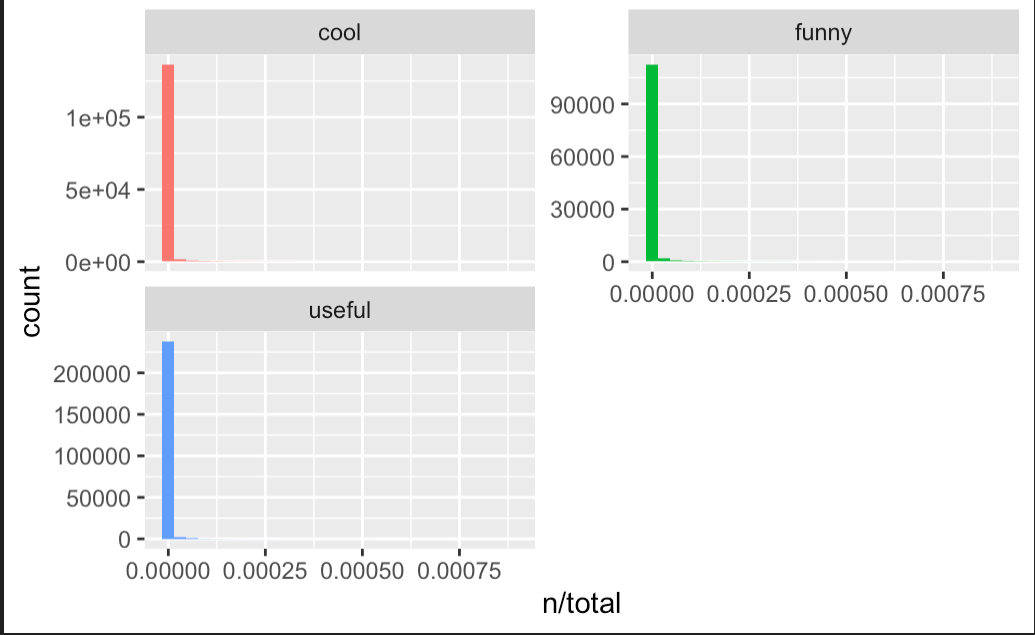
\includegraphics[scale=0.3]{histogram}

\end{frame}
% END


\end{document}
